\section{Разработка программного средства}

В данном раздела описывается процесс разработки программного \mbox{средства.}
\subsection{Обучение классификатора}
Правильная классификация черт личности является основной задачей данного проекта, результат зависит от предподготовки данных, процедуры оценки результата и финального качества обучения.

\begin{figure}[h]
    \centering
    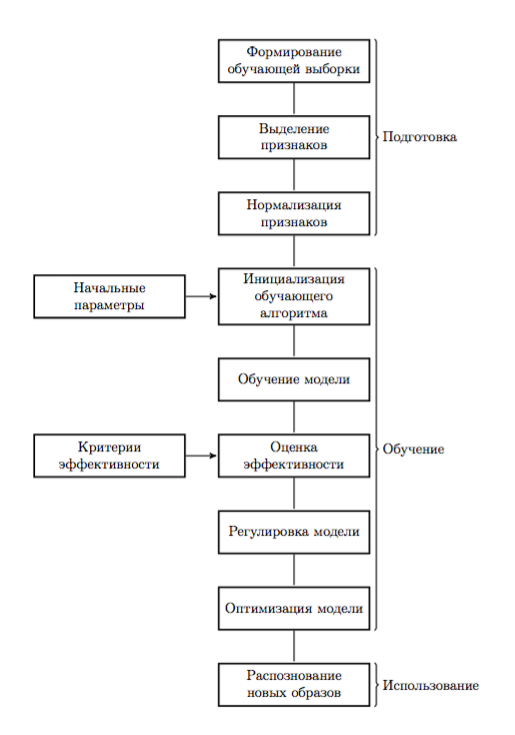
\includegraphics[width=0.7\textwidth]{figures/SVM_flow.png}
    \caption{Алгоритм обучения}
    \label{fig:develoipment:svm_flow}
\end{figure}

Общая схема подготовки, обучения и использования классификатора представлена на рисунке~\ref{fig:develoipment:svm_flow}.

После обучения классификатора можно переходить к классификации образов. В листинге~\ref{listing:development:classification} представлен метод классификации нового образца почерка на основе обученной модели. Всего в программном средстве различается 16 типов личности определяющих характеристики.

\lstinputlisting[
    style=commonstyle,
    caption=Метод классификации личности по параметрам почерка,
    label=listing:development:classification
]{src/evaluate_single_instance.java}

Для обучения классификатора будет использоваться обучающая выборка <<IAM Handwriting Database>>~\cite{IAM_handwriting_database} состоящая из 1539 образцов текста, написанных 500 авторами, с заранее выделенными параметрами почерка либо на основании выделенных параметров можно рассчитать параметры используемые в данной работе. Образцы почерка представлены изображениями в формате png, а параметры XML документом, пример параметров представлен в листинге~\ref{listing:development:sample_set}.
\lstinputlisting[
    style=commonstyle,
    caption=Пример XML-документа описывающего параметры почерка,
    label=listing:development:sample_set
]{src/sample_set.xml}

Данный объем и содержание обучающей выборки позволяет добиться хорошего качества классификации после обучения благодаря репрезентативности, в частности максимальная разность в количестве образцов разных классов составляет 13\%.

\subsection{Иерархия классов}
\begin{figure}[!ht]
    \centering
    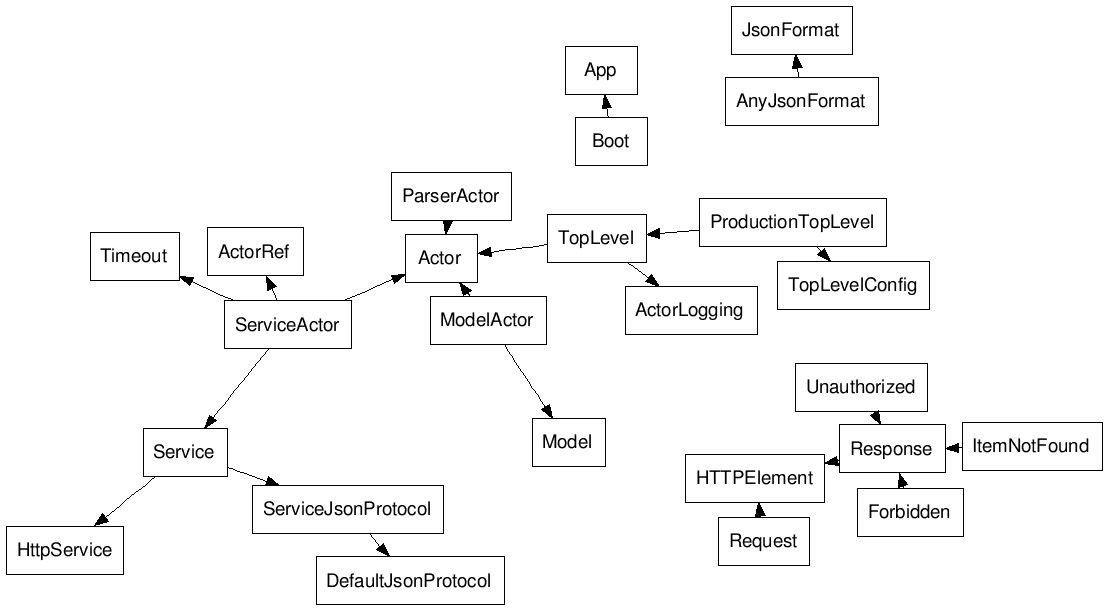
\includegraphics[width=1\textwidth]{figures/classes-fdp.png}
    \caption{Иерархия классов}
    \label{fig:develoipment:class_fdp}
\end{figure}

Общая диаграмма иерархии классов представлена на рисунке~\ref{fig:develoipment:class_fdp}. Все классы отвечающие за обработку запросов и данных, в частности \emph{ModelActor}, \emph{ParserActor}, \emph{ServiceActor} являются наследниками класса \emph{Actor} библиотека Akka. Это свидетельствует о том, что обработка информации на всех уровнях приложения происходит асинхронно.

Классы \emph{ItemNotFound}, \emph{Forbidden}, \emph{Unauthorized} являются наследниками класса \emph{Response} и представляют собой обертки для HTTP ответов на различные ошибочные ситуации на стороне клиента.

Классы \emph{ProductionTopLevel}, \emph{TopLevel} и \emph{TopLevelConfig} позволяют реализовать механизм управления зависимостями называемый \emph{Cake pattern}. При данном подходе все зависимости модуля, интерфейсы которые он использует в работе, перечисляются в специальной секции. Достоинствами данного подходя является полная поддержка средствами языка и проверка зависимостей на этапе компиляции.

Приведенная диаграмма является обобщенной диаграммой каждого модуля и представленные в ней элементы и связи справедливы для всех сервисов разработанного программного средства. Различия заключается лишь в функциях классов сервиса, например \emph{ModelActor} в сервисе доступа к базе данных отвечает за общение с базой данных, а в сервисе определения параметров личности за локальный кеш признаков образца.

Общая структура разделения кода на классы в каждом модуле позволит упростить понимания взаимодействия классов внутри всех модулей после изучения кода хотя бы одного из них.

\subsection{Маршрутизация запросов}
Библиотека Spray, описанная в пункте~\ref{sec:techs:spray}, имеет очень выразительный внутренний язык описания разбора, обработки и маршрутизации запросов к сервису. Модуль доступа к данным является связующий звеном между модулями приложения и базой данных. Поскольку одной из задач программного средства является предотвращение не авторизированного доступа к данным. Каждый обработчик запросов содержит секцию отвечающую за проверку прав доступа.
\lstinputlisting[
    style=commonstyle, 
    caption=Маршрутизация запросов к серверу в модуле доступа к данным,
    label=listing:development:db_rout
]{src/routing.scala}
Конструкция \emph{authorizeToken} описанная в модуле \emph{spray-jwt} отвечает за проверку прав доступа, подробнее будет рассмотрена в разделе~\ref{sec:development:access_control}, а \emph{path} отвечает за маршрутизацию и разбор параметров запросов. 

Использование высоко-интегрированных компонентов, таких как \emph{spray-jwt} позволяет снизить риски некорректной работы при обновлении версий одного из компонентов и ускорить разработку и сопровождения благодаря использованию схожих концепций и стиля разработки.

\subsection{Хранение данных}
Для хранения учетных и пользовательских данных используется СУБД MongoDB. Условно все данные можно разделить на образцы изображений, листинг~\ref{listing:development:json:sample} и описание пользовательских данных, листинг~\ref{listing:development:json:user}. Для хранения используется формат JSON что упрощает преобразование информации при общения сервисов между собой и с клиентом. 

\lstinputlisting[
    style=commonstyle,
    caption=Пример JSON-документа описывающего образец текста,
    label=listing:development:json:sample
]{src/sample_item.json}

\lstinputlisting[
    style=commonstyle,
    caption=Пример JSON-документа описывающего пользователя,
    label=listing:development:json:user
]{src/user_item.json}

\subsection{Контроль доступа}
\label{sec:development:access_control}
Для контроля доступа используется механизм основанный на использовании JWT-маркера. Основой данного подхода является использование асинхронной криптографии для подписи и проверки JWT-маркера и доверее информации хранящейся в нем. Для подписи используется алгоритм RSA.

В разрабатываемом программное средстве для обеспечение создания, подписи и проверки JWT-маркеров используется модуль \emph{spray-jwt}. Модуль авторизации после после сравнения имени пользователя и пароля с авторизационных данными хранящимися в базе, создает новый JWT-маркер содержащий уникальный идентификатор пользователя, алгоритм подписи, срок действия, тип маркера, а так же информацию о том является ли он администратором. Далее модуль авторизации подписывает созданный маркер своим секретным ключом и добавляет подпись к маркеру. Так же есть возможность передавать отрытый ключ для его проверки в теле маркера.
Финальное содержание JWT-маркера представлено в листинге~\ref{listing:development:jwt_token}. Далее весь маркер переводится в кодировку Base64, части маркера разделяются точкой, и прикрепляется к ответу клиента.
\lstinputlisting[
    style=commonstyle,
    caption=Пример JWT-маркера,
    label=listing:development:jwt_token
]{src/jwt_token.json}

Клиент получив JWT-маркер использует его для подтверждения прав доступа при запросам к сервисам входящим в состав программного средства прикрепляя его к запросам.

Каждый из сервисов приложения имеет открытый ключ, являющийся парным к закрытому ключу сервиса авторизации, для проверки подлинности подписи маркера. После чего данные содержащиеся в теле маркера могут быть использованы в работе, так как их подлинность доказана. Такой подход позволяет снизить нагрузку на сервис авторизации благодаря возможности сервисов самостоятельно осуществлять проверку подлинности маркера.

\subsection{Сборка и развертывание}
Для получения последнюю версию исходного кода программного средства используйте команду <<git clone>> в корневом каталоге ПС. Разрешение зависимостей, сборка и развертывание программного средства выполняется с помощью автоматической системы сборки sbt~\cite{sbt}, поэтому перед началом сборки необходимо установить данный инструмент. Программное средство в своей работе использует ряд библиотек. При помощи команды <<sbt>> в корневом каталоге ПС будет произведены загрузка всех необходимых библиотек включая компилятор языка Scala, а так же компиляция модуля программного средства.
Для развертывания модуля программного средства необходимо указать параметры развертывания в файле \emph{application.conf}, подробнее об этом рассказывается в главе~\ref{sec:manpage:admin_man}, и выполнить команду <<sbt run>>. Процесс сборки и развертывания практически полностью выполняется автоматически и не должен вызвать проблем.

Помимо этого сборка и развертывание приложения на тестовом окружении осуществляется автоматически при внесении изменений в базу исходного кода командой <<git push>>.

В данном разделе была рассмотрена общая структура обучение классификатора на основе метода опорных векторов, диаграмма иерархии классов разработанного программного средства, формата хранения внутрих данных приложения, таких как учетные записи пользователей и образцы почерка, а так же внешние данные, обучающую выборку. На данном этапе разработка и отладка программное средства закончена и можно переходи к его тестированию.